\chapter{Dynamisches Programmieren}

  \TODO{Hier fehlt noch etwas}
  
  \marginpar{15.5.12}
  
  \TODO{Hier fehlt noch etwas}
  
  \begin{lemma}
    Sei \(\alpha \leq 1/2\). Dann gilt \[ \sum_{i=0}^{\alpha \cdot n} \binom{n}{i} = O^*( 2^{h(\alpha) \cdot n} ), \] wobei \(h(\alpha) = - \alpha \log_2 \alpha - (1-\alpha) \log_2(1 - \alpha)\).
  \end{lemma}
  
  \begin{figure}[h]
    \centering
    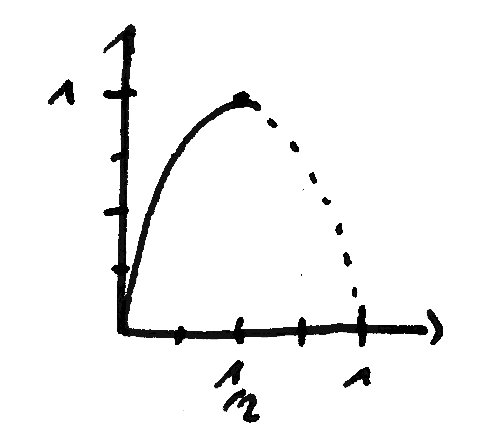
\includegraphics[width=.25\textwidth]{./Bilder/b01.jpg}
    % b01.jpg: 495x434 pixel, 72dpi, 17.46x15.31 cm, bb=0 0 495 434
    \caption{Graph des Binomialkoeffizienten}
  \end{figure}
  
  \begin{proof}
    Es ist \( \sum_{i=0}^{\alpha n} \leq n \binom{n}{\alpha n} = O^*( \binom{n}{\alpha n} ) \), denn die Binomialkoeffizienten \( \binom{a}{b} \) steigen für \(b \leq n/2\) monoton an. Per Definition gilt 
    \[
      \binom{n}{k} = \frac{n!}{k! (n-k)!}.
    \]
    Die Fakultät kann abgeschätzt werden durch \( \sqrt{2 \pi n} (n/e)^n \leq n! \leq 2 \sqrt{2 \pi n} (n/e)^n \), also ist \(n!\) proportional zu \((n/e)^n\). Daraus folgt, dass 
    \begin{eqnarray*}
      \binom{n}{\alpha n} &=& O^* \left( \frac{(n/e)^n}{(\alpha n/e)^{\alpha n} ( (1-\alpha)n/e)^{(1-\alpha) n}} \right) = O^* \left( \alpha^{-\alpha n} (1-\alpha)^{-(1-\alpha)n} \right) \\
      &=& O^* \left( 2^{-\alpha \log_2 \alpha n} \cdot 2^{-(1 - \alpha) \log_2(1-\alpha)n} \right),
    \end{eqnarray*}
    woraus die Behauptung folgt.
  \end{proof}
  
  \begin{theorem}
    Eine kleinste dominierende Mänge lässt sich in \(O(1,7088^n)\) ermitteln.
  \end{theorem}
  
  \begin{proof}
    Zunächst bestimmen wir eine nicht-erweiterbare unabhänge Menge \(I\). 
    Falls \(|I| \leq \alpha n\), testen wir in \(O^*(2^{h(\alpha) n})\) alle Teilmengen \(D \subseteq V\) mit \(|D| \leq |I|\).
    Falls \(|I| > \alpha n\), wende Satz \ref{satz??} an und berechne kleinste dominierende Menge in \(O^*(2^{(1-\alpha)n})\). % Satz in dem O*(2^(n-|I|)) bewiesen wurde
    
    \begin{figure}[h]
      \centering
      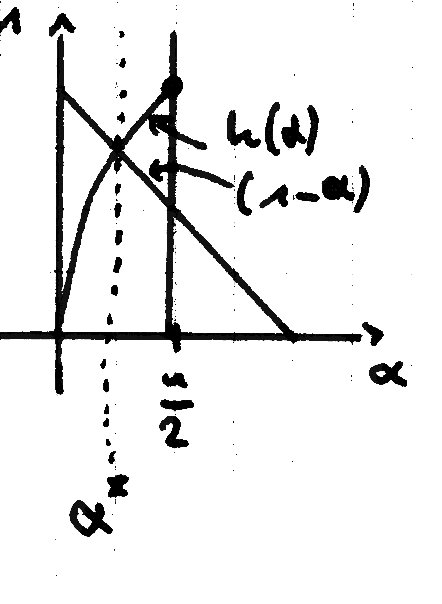
\includegraphics[width=.25\textwidth]{./Bilder/b02.jpg}
      % b02.jpg: 442x604 pixel, 72dpi, 15.59x21.31 cm, bb=0 0 442 604
      \caption{Bestimmung von \(\alpha^*\) als Maximum der zwei möglichen Funktionen}
    \end{figure}
    
    Aus der Skizze ergibt sich die Laufzeit als das Maximum der beiden dargestellten Funktionen bei \(\alpha^* \leq 0,22711\) bzw. \(O(2^{0,7729n}) = O(1,7088^n)\).
  \end{proof}
  
  Der schnellste derzeit bekannte Algorithmus für dieses Problem benötigt ca. \(O(1,5^n)\) und stammt aus 2010.



